\documentclass[1p]{elsarticle_modified}
%\bibliographystyle{elsarticle-num}

%\usepackage[colorlinks]{hyperref}
%\usepackage{abbrmath_seonhwa} %\Abb, \Ascr, \Acal ,\Abf, \Afrak
\usepackage{amsfonts}
\usepackage{amssymb}
\usepackage{amsmath}
\usepackage{amsthm}
\usepackage{scalefnt}
\usepackage{amsbsy}
\usepackage{kotex}
\usepackage{caption}
\usepackage{subfig}
\usepackage{color}
\usepackage{graphicx}
\usepackage{xcolor} %% white, black, red, green, blue, cyan, magenta, yellow
\usepackage{float}
\usepackage{setspace}
\usepackage{hyperref}

\usepackage{tikz}
\usetikzlibrary{arrows}

\usepackage{multirow}
\usepackage{array} % fixed length table
\usepackage{hhline}

%%%%%%%%%%%%%%%%%%%%%
\makeatletter
\renewcommand*\env@matrix[1][\arraystretch]{%
	\edef\arraystretch{#1}%
	\hskip -\arraycolsep
	\let\@ifnextchar\new@ifnextchar
	\array{*\c@MaxMatrixCols c}}
\makeatother %https://tex.stackexchange.com/questions/14071/how-can-i-increase-the-line-spacing-in-a-matrix
%%%%%%%%%%%%%%%

\usepackage[normalem]{ulem}

\newcommand{\msout}[1]{\ifmmode\text{\sout{\ensuremath{#1}}}\else\sout{#1}\fi}
%SOURCE: \msout is \stkout macro in https://tex.stackexchange.com/questions/20609/strikeout-in-math-mode

\newcommand{\cancel}[1]{
	\ifmmode
	{\color{red}\msout{#1}}
	\else
	{\color{red}\sout{#1}}
	\fi
}

\newcommand{\add}[1]{
	{\color{blue}\uwave{#1}}
}

\newcommand{\replace}[2]{
	\ifmmode
	{\color{red}\msout{#1}}{\color{blue}\uwave{#2}}
	\else
	{\color{red}\sout{#1}}{\color{blue}\uwave{#2}}
	\fi
}

\newcommand{\Sol}{\mathcal{S}} %segment
\newcommand{\D}{D} %diagram
\newcommand{\A}{\mathcal{A}} %arc


%%%%%%%%%%%%%%%%%%%%%%%%%%%%%5 test

\def\sl{\operatorname{\textup{SL}}(2,\Cbb)}
\def\psl{\operatorname{\textup{PSL}}(2,\Cbb)}
\def\quan{\mkern 1mu \triangleright \mkern 1mu}

\theoremstyle{definition}
\newtheorem{thm}{Theorem}[section]
\newtheorem{prop}[thm]{Proposition}
\newtheorem{lem}[thm]{Lemma}
\newtheorem{ques}[thm]{Question}
\newtheorem{cor}[thm]{Corollary}
\newtheorem{defn}[thm]{Definition}
\newtheorem{exam}[thm]{Example}
\newtheorem{rmk}[thm]{Remark}
\newtheorem{alg}[thm]{Algorithm}

\newcommand{\I}{\sqrt{-1}}
\begin{document}

%\begin{frontmatter}
%
%\title{Boundary parabolic representations of knots up to 8 crossings}
%
%%% Group authors per affiliation:
%\author{Yunhi Cho} 
%\address{Department of Mathematics, University of Seoul, Seoul, Korea}
%\ead{yhcho@uos.ac.kr}
%
%
%\author{Seonhwa Kim} %\fnref{s_kim}}
%\address{Center for Geometry and Physics, Institute for Basic Science, Pohang, 37673, Korea}
%\ead{ryeona17@ibs.re.kr}
%
%\author{Hyuk Kim}
%\address{Department of Mathematical Sciences, Seoul National University, Seoul 08826, Korea}
%\ead{hyukkim@snu.ac.kr}
%
%\author{Seokbeom Yoon}
%\address{Department of Mathematical Sciences, Seoul National University, Seoul, 08826,  Korea}
%\ead{sbyoon15@snu.ac.kr}
%
%\begin{abstract}
%We find all boundary parabolic representation of knots up to 8 crossings.
%
%\end{abstract}
%\begin{keyword}
%    \MSC[2010] 57M25 
%\end{keyword}
%
%\end{frontmatter}

%\linenumbers
%\tableofcontents
%
\newcommand\colored[1]{\textcolor{white}{\rule[-0.35ex]{0.8em}{1.4ex}}\kern-0.8em\color{red} #1}%
%\newcommand\colored[1]{\textcolor{white}{ #1}\kern-2.17ex	\textcolor{white}{ #1}\kern-1.81ex	\textcolor{white}{ #1}\kern-2.15ex\color{red}#1	}

{\Large $\underline{12n_{0228}~(K12n_{0228})}$}

\setlength{\tabcolsep}{10pt}
\renewcommand{\arraystretch}{1.6}
\vspace{1cm}\begin{tabular}{m{100pt}>{\centering\arraybackslash}m{274pt}}
\multirow{5}{120pt}{
	\centering
	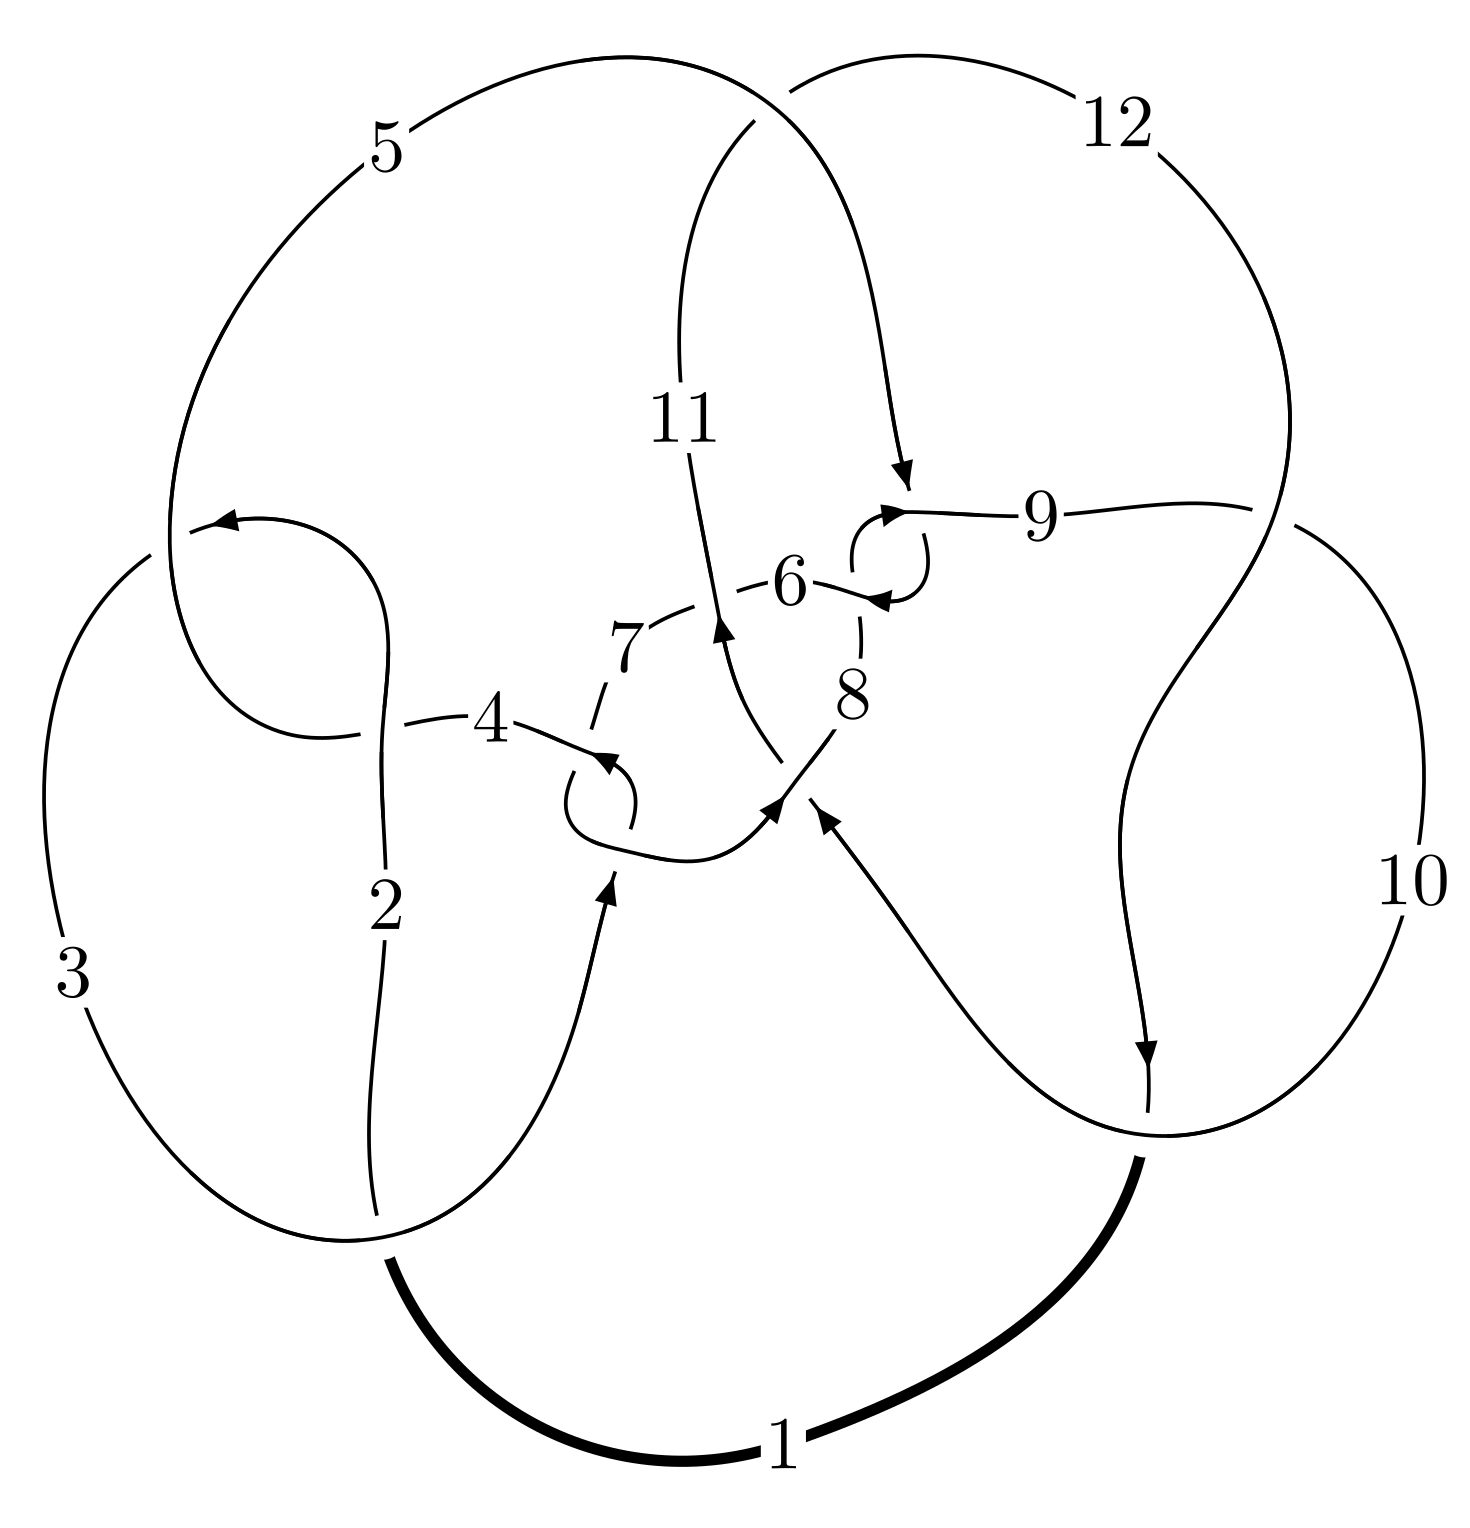
\includegraphics[width=112pt]{../../../GIT/diagram.site/Diagrams/png/2317_12n_0228.png}\\
\ \ \ A knot diagram\footnotemark}&
\allowdisplaybreaks
\textbf{Linearized knot diagam} \\
\cline{2-2}
 &
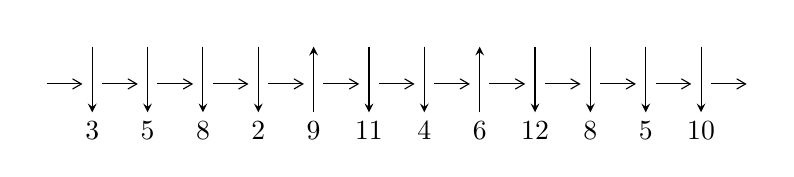
\begin{tikzpicture}[x=20pt, y=17pt]
	% nodes
	\node (C0) at (0, 0) {};
	\node (C1) at (1, 0) {};
	\node (C1U) at (1, +1) {};
	\node (C1D) at (1, -1) {3};

	\node (C2) at (2, 0) {};
	\node (C2U) at (2, +1) {};
	\node (C2D) at (2, -1) {5};

	\node (C3) at (3, 0) {};
	\node (C3U) at (3, +1) {};
	\node (C3D) at (3, -1) {8};

	\node (C4) at (4, 0) {};
	\node (C4U) at (4, +1) {};
	\node (C4D) at (4, -1) {2};

	\node (C5) at (5, 0) {};
	\node (C5U) at (5, +1) {};
	\node (C5D) at (5, -1) {9};

	\node (C6) at (6, 0) {};
	\node (C6U) at (6, +1) {};
	\node (C6D) at (6, -1) {11};

	\node (C7) at (7, 0) {};
	\node (C7U) at (7, +1) {};
	\node (C7D) at (7, -1) {4};

	\node (C8) at (8, 0) {};
	\node (C8U) at (8, +1) {};
	\node (C8D) at (8, -1) {6};

	\node (C9) at (9, 0) {};
	\node (C9U) at (9, +1) {};
	\node (C9D) at (9, -1) {12};

	\node (C10) at (10, 0) {};
	\node (C10U) at (10, +1) {};
	\node (C10D) at (10, -1) {8};

	\node (C11) at (11, 0) {};
	\node (C11U) at (11, +1) {};
	\node (C11D) at (11, -1) {5};

	\node (C12) at (12, 0) {};
	\node (C12U) at (12, +1) {};
	\node (C12D) at (12, -1) {10};
	\node (C13) at (13, 0) {};

	% arrows
	\draw[->,>={angle 60}]
	(C0) edge (C1) (C1) edge (C2) (C2) edge (C3) (C3) edge (C4) (C4) edge (C5) (C5) edge (C6) (C6) edge (C7) (C7) edge (C8) (C8) edge (C9) (C9) edge (C10) (C10) edge (C11) (C11) edge (C12) (C12) edge (C13) ;	\draw[->,>=stealth]
	(C1U) edge (C1D) (C2U) edge (C2D) (C3U) edge (C3D) (C4U) edge (C4D) (C5D) edge (C5U) (C6U) edge (C6D) (C7U) edge (C7D) (C8D) edge (C8U) (C9U) edge (C9D) (C10U) edge (C10D) (C11U) edge (C11D) (C12U) edge (C12D) ;
	\end{tikzpicture} \\
\hhline{~~} \\& 
\textbf{Solving Sequence} \\ \cline{2-2} 
 &
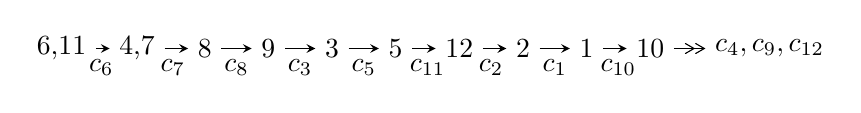
\begin{tikzpicture}[x=23pt, y=7pt]
	% node
	\node (A0) at (-1/8, 0) {6,11};
	\node (A1) at (17/16, 0) {4,7};
	\node (A2) at (17/8, 0) {8};
	\node (A3) at (25/8, 0) {9};
	\node (A4) at (33/8, 0) {3};
	\node (A5) at (41/8, 0) {5};
	\node (A6) at (49/8, 0) {12};
	\node (A7) at (57/8, 0) {2};
	\node (A8) at (65/8, 0) {1};
	\node (A9) at (73/8, 0) {10};
	\node (C1) at (1/2, -1) {$c_{6}$};
	\node (C2) at (13/8, -1) {$c_{7}$};
	\node (C3) at (21/8, -1) {$c_{8}$};
	\node (C4) at (29/8, -1) {$c_{3}$};
	\node (C5) at (37/8, -1) {$c_{5}$};
	\node (C6) at (45/8, -1) {$c_{11}$};
	\node (C7) at (53/8, -1) {$c_{2}$};
	\node (C8) at (61/8, -1) {$c_{1}$};
	\node (C9) at (69/8, -1) {$c_{10}$};
	\node (A10) at (11, 0) {$c_{4},c_{9},c_{12}$};

	% edge
	\draw[->,>=stealth]	
	(A0) edge (A1) (A1) edge (A2) (A2) edge (A3) (A3) edge (A4) (A4) edge (A5) (A5) edge (A6) (A6) edge (A7) (A7) edge (A8) (A8) edge (A9) ;
	\draw[->>,>={angle 60}]	
	(A9) edge (A10);
\end{tikzpicture} \\ 

\end{tabular} \\

\footnotetext{
The image of knot diagram is generated by the software ``\textbf{Draw programme}" developed by Andrew Bartholomew(\url{http://www.layer8.co.uk/maths/draw/index.htm\#Running-draw}), where we modified some parts for our purpose(\url{https://github.com/CATsTAILs/LinksPainter}).
}\phantom \\ \newline 
\centering \textbf{Ideals for irreducible components\footnotemark of $X_{\text{par}}$} 
 
\begin{align*}
I^u_{1}&=\langle 
-9861446311968 u^{17}+13967634545632 u^{16}+\cdots+5212485204695 b-26164458415624,\\
\phantom{I^u_{1}}&\phantom{= \langle  }-35356917620792 u^{17}+9192459205168 u^{16}+\cdots+5212485204695 a+53817437592104,\\
\phantom{I^u_{1}}&\phantom{= \langle  }u^{18}- u^{17}+\cdots- u-1\rangle \\
I^u_{2}&=\langle 
u^8+u^6+2 u^4+u^2+b+u,\;u^8+u^7+3 u^6+u^5+4 u^4+u^3+4 u^2+a+2,\\
\phantom{I^u_{2}}&\phantom{= \langle  }u^9+u^8+2 u^7+u^6+3 u^5+u^4+2 u^3+u-1\rangle \\
I^u_{3}&=\langle 
-1.81728\times10^{21} u^{17}+1.12182\times10^{21} u^{16}+\cdots+3.70892\times10^{24} b-2.85100\times10^{23},\\
\phantom{I^u_{3}}&\phantom{= \langle  }6.07558\times10^{21} u^{17}-6.65651\times10^{21} u^{16}+\cdots+3.70892\times10^{24} a-7.70911\times10^{24},\\
\phantom{I^u_{3}}&\phantom{= \langle  }u^{18}- u^{17}+\cdots-1024 u+512\rangle \\
\\
I^v_{1}&=\langle 
a,\;16726 v^8+41423 v^7+\cdots+11959 b+26601,\\
\phantom{I^v_{1}}&\phantom{= \langle  }v^9+3 v^8-2 v^7+6 v^6+25 v^5+11 v^4-9 v^3-2 v^2+3 v+1\rangle \\
\end{align*}
\raggedright * 4 irreducible components of $\dim_{\mathbb{C}}=0$, with total 54 representations.\\
\footnotetext{All coefficients of polynomials are rational numbers. But the coefficients are sometimes approximated in decimal forms when there is not enough margin.}
\newpage
\renewcommand{\arraystretch}{1}
\centering \section*{I. $I^u_{1}= \langle -9.86\times10^{12} u^{17}+1.40\times10^{13} u^{16}+\cdots+5.21\times10^{12} b-2.62\times10^{13},\;-3.54\times10^{13} u^{17}+9.19\times10^{12} u^{16}+\cdots+5.21\times10^{12} a+5.38\times10^{13},\;u^{18}- u^{17}+\cdots- u-1 \rangle$}
\flushleft \textbf{(i) Arc colorings}\\
\begin{tabular}{m{7pt} m{180pt} m{7pt} m{180pt} }
\flushright $a_{6}=$&$\begin{pmatrix}1\\0\end{pmatrix}$ \\
\flushright $a_{11}=$&$\begin{pmatrix}0\\u\end{pmatrix}$ \\
\flushright $a_{4}=$&$\begin{pmatrix}6.78312 u^{17}-1.76355 u^{16}+\cdots-14.7181 u-10.3247\\1.89189 u^{17}-2.67965 u^{16}+\cdots+10.8027 u+5.01957\end{pmatrix}$ \\
\flushright $a_{7}=$&$\begin{pmatrix}1\\u^2\end{pmatrix}$ \\
\flushright $a_{8}=$&$\begin{pmatrix}-5.01957 u^{17}+3.12769 u^{16}+\cdots+3.54160 u-5.78312\\0.787760 u^{17}+0.523498 u^{16}+\cdots-6.91146 u-1.89189\end{pmatrix}$ \\
\flushright $a_{9}=$&$\begin{pmatrix}-4.23181 u^{17}+3.65118 u^{16}+\cdots-3.36987 u-7.67501\\0.787760 u^{17}+0.523498 u^{16}+\cdots-6.91146 u-1.89189\end{pmatrix}$ \\
\flushright $a_{3}=$&$\begin{pmatrix}8.67501 u^{17}-4.44320 u^{16}+\cdots-3.91541 u-5.30514\\0.580631 u^{17}-1.87796 u^{16}+\cdots+11.9068 u+4.23181\end{pmatrix}$ \\
\flushright $a_{5}=$&$\begin{pmatrix}-0.182502 u^{17}-1.66573 u^{16}+\cdots+14.4199 u+6.60470\\-0.872414 u^{17}+0.452638 u^{16}+\cdots+1.36048 u-0.117197\end{pmatrix}$ \\
\flushright $a_{12}=$&$\begin{pmatrix}9.81987 u^{17}-10.3086 u^{16}+\cdots+26.3092 u+18.8999\\-2.15014 u^{17}-0.0100325 u^{16}+\cdots+10.2859 u+1.01350\end{pmatrix}$ \\
\flushright $a_{2}=$&$\begin{pmatrix}8.04847 u^{17}-1.60224 u^{16}+\cdots-21.8507 u-13.9296\\2.27885 u^{17}-3.00234 u^{16}+\cdots+11.9846 u+5.66748\end{pmatrix}$ \\
\flushright $a_{1}=$&$\begin{pmatrix}0.307849 u^{17}+0.749387 u^{16}+\cdots-5.26730 u-4.18442\\0.509570 u^{17}-0.575614 u^{16}+\cdots+2.09902 u+1.31126\end{pmatrix}$ \\
\flushright $a_{10}=$&$\begin{pmatrix}7.61379 u^{17}-7.71164 u^{16}+\cdots+21.1440 u+12.3571\\-1.42846 u^{17}+0.0464712 u^{16}+\cdots+7.41181 u+0.689913\end{pmatrix}$\\&\end{tabular}
\flushleft \textbf{(ii) Obstruction class $= -1$}\\~\\
\flushleft \textbf{(iii) Cusp Shapes $= \frac{33036266987992}{5212485204695} u^{17}-\frac{83885068578828}{5212485204695} u^{16}+\cdots+\frac{600947759550584}{5212485204695} u-\frac{154008499337594}{5212485204695}$}\\~\\
\newpage\renewcommand{\arraystretch}{1}
\flushleft \textbf{(iv) u-Polynomials at the component}\newline \\
\begin{tabular}{m{50pt}|m{274pt}}
Crossings & \hspace{64pt}u-Polynomials at each crossing \\
\hline $$\begin{aligned}c_{1}\end{aligned}$$&$\begin{aligned}
&u^{18}+11 u^{17}+\cdots+3 u+1
\end{aligned}$\\
\hline $$\begin{aligned}c_{2},c_{4},c_{9}\\c_{12}\end{aligned}$$&$\begin{aligned}
&u^{18}-7 u^{17}+\cdots- u+1
\end{aligned}$\\
\hline $$\begin{aligned}c_{3},c_{6},c_{7}\end{aligned}$$&$\begin{aligned}
&u^{18}+u^{17}+\cdots+u-1
\end{aligned}$\\
\hline $$\begin{aligned}c_{5},c_{8}\end{aligned}$$&$\begin{aligned}
&u^{18}+u^{17}+\cdots+3 u-1
\end{aligned}$\\
\hline $$\begin{aligned}c_{10}\end{aligned}$$&$\begin{aligned}
&u^{18}-3 u^{17}+\cdots+517 u-1
\end{aligned}$\\
\hline $$\begin{aligned}c_{11}\end{aligned}$$&$\begin{aligned}
&u^{18}-5 u^{17}+\cdots+77 u-23
\end{aligned}$\\
\hline
\end{tabular}\\~\\
\newpage\renewcommand{\arraystretch}{1}
\flushleft \textbf{(v) Riley Polynomials at the component}\newline \\
\begin{tabular}{m{50pt}|m{274pt}}
Crossings & \hspace{64pt}Riley Polynomials at each crossing \\
\hline $$\begin{aligned}c_{1}\end{aligned}$$&$\begin{aligned}
&y^{18}+41 y^{17}+\cdots-47 y+1
\end{aligned}$\\
\hline $$\begin{aligned}c_{2},c_{4},c_{9}\\c_{12}\end{aligned}$$&$\begin{aligned}
&y^{18}-11 y^{17}+\cdots-3 y+1
\end{aligned}$\\
\hline $$\begin{aligned}c_{3},c_{6},c_{7}\end{aligned}$$&$\begin{aligned}
&y^{18}+21 y^{17}+\cdots-7 y+1
\end{aligned}$\\
\hline $$\begin{aligned}c_{5},c_{8}\end{aligned}$$&$\begin{aligned}
&y^{18}+13 y^{17}+\cdots-43 y+1
\end{aligned}$\\
\hline $$\begin{aligned}c_{10}\end{aligned}$$&$\begin{aligned}
&y^{18}+29 y^{17}+\cdots-268915 y+1
\end{aligned}$\\
\hline $$\begin{aligned}c_{11}\end{aligned}$$&$\begin{aligned}
&y^{18}+y^{17}+\cdots-5331 y+529
\end{aligned}$\\
\hline
\end{tabular}\\~\\
\newpage\flushleft \textbf{(vi) Complex Volumes and Cusp Shapes}
$$\begin{array}{c|c|c}  
\text{Solutions to }I^u_{1}& \I (\text{vol} + \sqrt{-1}CS) & \text{Cusp shape}\\
 \hline 
\begin{aligned}
u &= -0.557323 + 0.726879 I \\
a &= -0.078908 - 0.132094 I \\
b &= \phantom{-}0.467481 - 0.634184 I\end{aligned}
 & -5.49927 + 7.93492 I & -11.8455 - 13.1993 I \\ \hline\begin{aligned}
u &= -0.557323 - 0.726879 I \\
a &= -0.078908 + 0.132094 I \\
b &= \phantom{-}0.467481 + 0.634184 I\end{aligned}
 & -5.49927 - 7.93492 I & -11.8455 + 13.1993 I \\ \hline\begin{aligned}
u &= -0.781322 + 0.060789 I \\
a &= -1.67426 - 2.33250 I \\
b &= -0.456133 - 1.317030 I\end{aligned}
 & -3.91966 - 2.10303 I & -13.59813 + 2.08848 I \\ \hline\begin{aligned}
u &= -0.781322 - 0.060789 I \\
a &= -1.67426 + 2.33250 I \\
b &= -0.456133 + 1.317030 I\end{aligned}
 & -3.91966 + 2.10303 I & -13.59813 - 2.08848 I \\ \hline\begin{aligned}
u &= \phantom{-}0.136626 + 0.709955 I \\
a &= \phantom{-}0.134891 + 0.049791 I \\
b &= -0.211757 - 0.707953 I\end{aligned}
 & \phantom{-}0.64686 - 2.83787 I & \phantom{-}0.86568 + 9.86296 I \\ \hline\begin{aligned}
u &= \phantom{-}0.136626 - 0.709955 I \\
a &= \phantom{-}0.134891 - 0.049791 I \\
b &= -0.211757 + 0.707953 I\end{aligned}
 & \phantom{-}0.64686 + 2.83787 I & \phantom{-}0.86568 - 9.86296 I \\ \hline\begin{aligned}
u &= \phantom{-}0.367491 + 0.554636 I \\
a &= -0.073321 + 0.530685 I \\
b &= -0.571171 - 0.676106 I\end{aligned}
 & -0.53975 - 1.77290 I & -3.88757 + 3.00933 I \\ \hline\begin{aligned}
u &= \phantom{-}0.367491 - 0.554636 I \\
a &= -0.073321 - 0.530685 I \\
b &= -0.571171 + 0.676106 I\end{aligned}
 & -0.53975 + 1.77290 I & -3.88757 - 3.00933 I \\ \hline\begin{aligned}
u &= \phantom{-}0.344494 + 0.511075 I \\
a &= \phantom{-}2.56907 - 7.38757 I \\
b &= \phantom{-}1.89070 + 1.44645 I\end{aligned}
 & -5.78192 + 0.83339 I & -4.3200 + 13.4737 I \\ \hline\begin{aligned}
u &= \phantom{-}0.344494 - 0.511075 I \\
a &= \phantom{-}2.56907 + 7.38757 I \\
b &= \phantom{-}1.89070 - 1.44645 I\end{aligned}
 & -5.78192 - 0.83339 I & -4.3200 - 13.4737 I\\
 \hline 
 \end{array}$$\newpage$$\begin{array}{c|c|c}  
\text{Solutions to }I^u_{1}& \I (\text{vol} + \sqrt{-1}CS) & \text{Cusp shape}\\
 \hline 
\begin{aligned}
u &= \phantom{-}0.604129\phantom{ +0.000000I} \\
a &= \phantom{-}1.66056\phantom{ +0.000000I} \\
b &= \phantom{-}0.00192836\phantom{ +0.000000I}\end{aligned}
 & -1.09450\phantom{ +0.000000I} & -7.23730\phantom{ +0.000000I} \\ \hline\begin{aligned}
u &= -0.318928\phantom{ +0.000000I} \\
a &= -11.2006\phantom{ +0.000000I} \\
b &= -0.820343\phantom{ +0.000000I}\end{aligned}
 & -3.03100\phantom{ +0.000000I} & -72.2820\phantom{ +0.000000I} \\ \hline\begin{aligned}
u &= \phantom{-}0.74883 + 1.97520 I \\
a &= \phantom{-}0.448418 - 0.789734 I \\
b &= \phantom{-}0.08933 + 1.98953 I\end{aligned}
 & \phantom{-}9.51613 - 3.71804 I & -9.22156 + 1.51475 I \\ \hline\begin{aligned}
u &= \phantom{-}0.74883 - 1.97520 I \\
a &= \phantom{-}0.448418 + 0.789734 I \\
b &= \phantom{-}0.08933 - 1.98953 I\end{aligned}
 & \phantom{-}9.51613 + 3.71804 I & -9.22156 - 1.51475 I \\ \hline\begin{aligned}
u &= -0.83783 + 2.05810 I \\
a &= -0.421019 - 0.873213 I \\
b &= -0.68580 + 2.47962 I\end{aligned}
 & \phantom{-}13.3797 + 9.0997 I & -6.48039 - 4.12934 I \\ \hline\begin{aligned}
u &= -0.83783 - 2.05810 I \\
a &= -0.421019 + 0.873213 I \\
b &= -0.68580 - 2.47962 I\end{aligned}
 & \phantom{-}13.3797 - 9.0997 I & -6.48039 + 4.12934 I \\ \hline\begin{aligned}
u &= \phantom{-}0.93643 + 2.07951 I \\
a &= \phantom{-}0.365142 - 0.919671 I \\
b &= \phantom{-}1.38656 + 2.51311 I\end{aligned}
 & \phantom{-}9.0651 - 14.3484 I & -9.75296 + 6.52825 I \\ \hline\begin{aligned}
u &= \phantom{-}0.93643 - 2.07951 I \\
a &= \phantom{-}0.365142 + 0.919671 I \\
b &= \phantom{-}1.38656 - 2.51311 I\end{aligned}
 & \phantom{-}9.0651 + 14.3484 I & -9.75296 - 6.52825 I\\
 \hline 
 \end{array}$$\newpage\newpage\renewcommand{\arraystretch}{1}
\centering \section*{II. $I^u_{2}= \langle u^8+u^6+2 u^4+u^2+b+u,\;u^8+u^7+3 u^6+u^5+4 u^4+u^3+4 u^2+a+2,\;u^9+u^8+2 u^7+u^6+3 u^5+u^4+2 u^3+u-1 \rangle$}
\flushleft \textbf{(i) Arc colorings}\\
\begin{tabular}{m{7pt} m{180pt} m{7pt} m{180pt} }
\flushright $a_{6}=$&$\begin{pmatrix}1\\0\end{pmatrix}$ \\
\flushright $a_{11}=$&$\begin{pmatrix}0\\u\end{pmatrix}$ \\
\flushright $a_{4}=$&$\begin{pmatrix}- u^8- u^7-3 u^6- u^5-4 u^4- u^3-4 u^2-2\\- u^8- u^6-2 u^4- u^2- u\end{pmatrix}$ \\
\flushright $a_{7}=$&$\begin{pmatrix}1\\u^2\end{pmatrix}$ \\
\flushright $a_{8}=$&$\begin{pmatrix}1\\u^2\end{pmatrix}$ \\
\flushright $a_{9}=$&$\begin{pmatrix}u^2+1\\u^2\end{pmatrix}$ \\
\flushright $a_{3}=$&$\begin{pmatrix}- u^8- u^7-3 u^6- u^5-4 u^4- u^3-4 u^2-2\\- u^8- u^6-2 u^4- u^2- u\end{pmatrix}$ \\
\flushright $a_{5}=$&$\begin{pmatrix}u^4+u^2+1\\u^4\end{pmatrix}$ \\
\flushright $a_{12}=$&$\begin{pmatrix}u^8+u^6+u^4-1\\u^8+u^7+u^6+2 u^5+u^4+2 u^3+2 u-1\end{pmatrix}$ \\
\flushright $a_{2}=$&$\begin{pmatrix}- u^8- u^7-3 u^6- u^5-5 u^4- u^3-5 u^2-3\\- u^8- u^6-3 u^4- u^2- u\end{pmatrix}$ \\
\flushright $a_{1}=$&$\begin{pmatrix}- u^4- u^2-1\\- u^4\end{pmatrix}$ \\
\flushright $a_{10}=$&$\begin{pmatrix}u\\u^3+u\end{pmatrix}$\\&\end{tabular}
\flushleft \textbf{(ii) Obstruction class $= 1$}\\~\\
\flushleft \textbf{(iii) Cusp Shapes $= 4 u^8+5 u^6+u^5+9 u^4+5 u^2+4 u-8$}\\~\\
\newpage\renewcommand{\arraystretch}{1}
\flushleft \textbf{(iv) u-Polynomials at the component}\newline \\
\begin{tabular}{m{50pt}|m{274pt}}
Crossings & \hspace{64pt}u-Polynomials at each crossing \\
\hline $$\begin{aligned}c_{1},c_{2}\end{aligned}$$&$\begin{aligned}
&(u-1)^9
\end{aligned}$\\
\hline $$\begin{aligned}c_{3},c_{7}\end{aligned}$$&$\begin{aligned}
&u^9
\end{aligned}$\\
\hline $$\begin{aligned}c_{4}\end{aligned}$$&$\begin{aligned}
&(u+1)^9
\end{aligned}$\\
\hline $$\begin{aligned}c_{5}\end{aligned}$$&$\begin{aligned}
&u^9+3 u^8+8 u^7+13 u^6+17 u^5+17 u^4+12 u^3+6 u^2+u-1
\end{aligned}$\\
\hline $$\begin{aligned}c_{6}\end{aligned}$$&$\begin{aligned}
&u^9+u^8+2 u^7+u^6+3 u^5+u^4+2 u^3+u-1
\end{aligned}$\\
\hline $$\begin{aligned}c_{8}\end{aligned}$$&$\begin{aligned}
&u^9-3 u^8+8 u^7-13 u^6+17 u^5-17 u^4+12 u^3-6 u^2+u+1
\end{aligned}$\\
\hline $$\begin{aligned}c_{9}\end{aligned}$$&$\begin{aligned}
&u^9+u^8-2 u^7-3 u^6+u^5+3 u^4+2 u^3- u-1
\end{aligned}$\\
\hline $$\begin{aligned}c_{10}\end{aligned}$$&$\begin{aligned}
&u^9- u^8+2 u^7- u^6+3 u^5- u^4+2 u^3+u+1
\end{aligned}$\\
\hline $$\begin{aligned}c_{11}\end{aligned}$$&$\begin{aligned}
&u^9+5 u^8+12 u^7+15 u^6+9 u^5- u^4-4 u^3-2 u^2+u+1
\end{aligned}$\\
\hline $$\begin{aligned}c_{12}\end{aligned}$$&$\begin{aligned}
&u^9- u^8-2 u^7+3 u^6+u^5-3 u^4+2 u^3- u+1
\end{aligned}$\\
\hline
\end{tabular}\\~\\
\newpage\renewcommand{\arraystretch}{1}
\flushleft \textbf{(v) Riley Polynomials at the component}\newline \\
\begin{tabular}{m{50pt}|m{274pt}}
Crossings & \hspace{64pt}Riley Polynomials at each crossing \\
\hline $$\begin{aligned}c_{1},c_{2},c_{4}\end{aligned}$$&$\begin{aligned}
&(y-1)^9
\end{aligned}$\\
\hline $$\begin{aligned}c_{3},c_{7}\end{aligned}$$&$\begin{aligned}
&y^9
\end{aligned}$\\
\hline $$\begin{aligned}c_{5},c_{8}\end{aligned}$$&$\begin{aligned}
&y^9+7 y^8+20 y^7+25 y^6+5 y^5-15 y^4+22 y^2+13 y-1
\end{aligned}$\\
\hline $$\begin{aligned}c_{6},c_{10}\end{aligned}$$&$\begin{aligned}
&y^9+3 y^8+8 y^7+13 y^6+17 y^5+17 y^4+12 y^3+6 y^2+y-1
\end{aligned}$\\
\hline $$\begin{aligned}c_{9},c_{12}\end{aligned}$$&$\begin{aligned}
&y^9-5 y^8+12 y^7-15 y^6+9 y^5+y^4-4 y^3+2 y^2+y-1
\end{aligned}$\\
\hline $$\begin{aligned}c_{11}\end{aligned}$$&$\begin{aligned}
&y^9- y^8+12 y^7-7 y^6+37 y^5+y^4-10 y^2+5 y-1
\end{aligned}$\\
\hline
\end{tabular}\\~\\
\newpage\flushleft \textbf{(vi) Complex Volumes and Cusp Shapes}
$$\begin{array}{c|c|c}  
\text{Solutions to }I^u_{2}& \I (\text{vol} + \sqrt{-1}CS) & \text{Cusp shape}\\
 \hline 
\begin{aligned}
u &= \phantom{-}0.140343 + 0.966856 I \\
a &= \phantom{-}0.483566 + 0.305056 I \\
b &= -0.525305 - 0.147929 I\end{aligned}
 & \phantom{-}0.13850 - 2.09337 I & -6.02684 + 1.69698 I \\ \hline\begin{aligned}
u &= \phantom{-}0.140343 - 0.966856 I \\
a &= \phantom{-}0.483566 - 0.305056 I \\
b &= -0.525305 + 0.147929 I\end{aligned}
 & \phantom{-}0.13850 + 2.09337 I & -6.02684 - 1.69698 I \\ \hline\begin{aligned}
u &= \phantom{-}0.628449 + 0.875112 I \\
a &= -1.022450 + 0.246780 I \\
b &= \phantom{-}0.107759 - 1.216140 I\end{aligned}
 & -2.26187 - 2.45442 I & -8.53903 + 2.82066 I \\ \hline\begin{aligned}
u &= \phantom{-}0.628449 - 0.875112 I \\
a &= -1.022450 - 0.246780 I \\
b &= \phantom{-}0.107759 + 1.216140 I\end{aligned}
 & -2.26187 + 2.45442 I & -8.53903 - 2.82066 I \\ \hline\begin{aligned}
u &= -0.796005 + 0.733148 I \\
a &= \phantom{-}1.23246 + 1.62704 I \\
b &= \phantom{-}2.01751 - 1.28212 I\end{aligned}
 & -6.01628 - 1.33617 I & -16.4774 + 4.4812 I \\ \hline\begin{aligned}
u &= -0.796005 - 0.733148 I \\
a &= \phantom{-}1.23246 - 1.62704 I \\
b &= \phantom{-}2.01751 + 1.28212 I\end{aligned}
 & -6.01628 + 1.33617 I & -16.4774 - 4.4812 I \\ \hline\begin{aligned}
u &= -0.728966 + 0.986295 I \\
a &= -0.411691 + 0.129409 I \\
b &= \phantom{-}0.367799 + 0.534872 I\end{aligned}
 & -5.24306 + 7.08493 I & -9.02021 - 2.94778 I \\ \hline\begin{aligned}
u &= -0.728966 - 0.986295 I \\
a &= -0.411691 - 0.129409 I \\
b &= \phantom{-}0.367799 - 0.534872 I\end{aligned}
 & -5.24306 - 7.08493 I & -9.02021 + 2.94778 I \\ \hline\begin{aligned}
u &= \phantom{-}0.512358\phantom{ +0.000000I} \\
a &= -3.56378\phantom{ +0.000000I} \\
b &= -0.935531\phantom{ +0.000000I}\end{aligned}
 & -2.84338\phantom{ +0.000000I} & -3.87310\phantom{ +0.000000I}\\
 \hline 
 \end{array}$$\newpage\newpage\renewcommand{\arraystretch}{1}
\centering \section*{III. $I^u_{3}= \langle -1.82\times10^{21} u^{17}+1.12\times10^{21} u^{16}+\cdots+3.71\times10^{24} b-2.85\times10^{23},\;6.08\times10^{21} u^{17}-6.66\times10^{21} u^{16}+\cdots+3.71\times10^{24} a-7.71\times10^{24},\;u^{18}- u^{17}+\cdots-1024 u+512 \rangle$}
\flushleft \textbf{(i) Arc colorings}\\
\begin{tabular}{m{7pt} m{180pt} m{7pt} m{180pt} }
\flushright $a_{6}=$&$\begin{pmatrix}1\\0\end{pmatrix}$ \\
\flushright $a_{11}=$&$\begin{pmatrix}0\\u\end{pmatrix}$ \\
\flushright $a_{4}=$&$\begin{pmatrix}-0.00163810 u^{17}+0.00179473 u^{16}+\cdots-2.49995 u+2.07853\\0.000489974 u^{17}-0.000302464 u^{16}+\cdots-1.00081 u+0.0768688\end{pmatrix}$ \\
\flushright $a_{7}=$&$\begin{pmatrix}1\\u^2\end{pmatrix}$ \\
\flushright $a_{8}=$&$\begin{pmatrix}-0.000647148 u^{17}+0.00137895 u^{16}+\cdots-2.62281 u-0.193950\\-0.000380983 u^{17}+0.000549244 u^{16}+\cdots-1.73916 u+0.608978\end{pmatrix}$ \\
\flushright $a_{9}=$&$\begin{pmatrix}-0.00102813 u^{17}+0.00192819 u^{16}+\cdots-4.36197 u+0.415028\\-0.000380983 u^{17}+0.000549244 u^{16}+\cdots-1.73916 u+0.608978\end{pmatrix}$ \\
\flushright $a_{3}=$&$\begin{pmatrix}-0.00322523 u^{17}+0.00350611 u^{16}+\cdots-2.41456 u+1.38902\\-0.0000152880 u^{17}+0.000660040 u^{16}+\cdots-2.70270 u+0.0251916\end{pmatrix}$ \\
\flushright $a_{5}=$&$\begin{pmatrix}-0.00137194 u^{17}+0.000914778 u^{16}+\cdots+3.57480 u-0.897464\\-0.000606358 u^{17}+0.000539657 u^{16}+\cdots+0.359893 u-0.400830\end{pmatrix}$ \\
\flushright $a_{12}=$&$\begin{pmatrix}-0.00177283 u^{17}+0.00280042 u^{16}+\cdots-7.34159 u+0.997270\\-0.000412612 u^{17}+0.000733802 u^{16}+\cdots-2.73715 u+0.865009\end{pmatrix}$ \\
\flushright $a_{2}=$&$\begin{pmatrix}-0.000957173 u^{17}+0.00142033 u^{16}+\cdots-4.42822 u+2.32273\\0.000900583 u^{17}-0.000630850 u^{16}+\cdots-1.88345 u+0.230042\end{pmatrix}$ \\
\flushright $a_{1}=$&$\begin{pmatrix}0.00197317 u^{17}-0.00315915 u^{16}+\cdots+8.61298 u-1.34243\\0.000666946 u^{17}-0.000742761 u^{16}+\cdots+3.18723 u-1.06981\end{pmatrix}$ \\
\flushright $a_{10}=$&$\begin{pmatrix}-0.00115375 u^{17}+0.00192948 u^{16}+\cdots-2.60407 u+0.0364046\\-0.000390462 u^{17}+0.000755167 u^{16}+\cdots-1.28059 u+0.391978\end{pmatrix}$\\&\end{tabular}
\flushleft \textbf{(ii) Obstruction class $= -1$}\\~\\
\flushleft \textbf{(iii) Cusp Shapes $= -\frac{335010846082545701}{542874601956974270032} u^{17}+\frac{62587569732089869}{4342996815655794160256} u^{16}+\cdots+\frac{240047666391711939473}{67859325244621783754} u-\frac{317868067795007140580}{33929662622310891877}$}\\~\\
\newpage\renewcommand{\arraystretch}{1}
\flushleft \textbf{(iv) u-Polynomials at the component}\newline \\
\begin{tabular}{m{50pt}|m{274pt}}
Crossings & \hspace{64pt}u-Polynomials at each crossing \\
\hline $$\begin{aligned}c_{1}\end{aligned}$$&$\begin{aligned}
&u^{18}-10 u^{17}+\cdots+18 u+1
\end{aligned}$\\
\hline $$\begin{aligned}c_{2},c_{4},c_{9}\\c_{12}\end{aligned}$$&$\begin{aligned}
&u^{18}-4 u^{17}+\cdots-9 u^2+1
\end{aligned}$\\
\hline $$\begin{aligned}c_{3},c_{6},c_{7}\end{aligned}$$&$\begin{aligned}
&u^{18}+u^{17}+\cdots+1024 u+512
\end{aligned}$\\
\hline $$\begin{aligned}c_{5},c_{8}\end{aligned}$$&$\begin{aligned}
&(u^9+u^8+4 u^7+3 u^6+5 u^5+3 u^4-3 u-1)^2
\end{aligned}$\\
\hline $$\begin{aligned}c_{10}\end{aligned}$$&$\begin{aligned}
&u^{18}+4 u^{17}+\cdots+1179 u-199
\end{aligned}$\\
\hline $$\begin{aligned}c_{11}\end{aligned}$$&$\begin{aligned}
&u^{18}-3 u^{17}+\cdots+3241 u+1303
\end{aligned}$\\
\hline
\end{tabular}\\~\\
\newpage\renewcommand{\arraystretch}{1}
\flushleft \textbf{(v) Riley Polynomials at the component}\newline \\
\begin{tabular}{m{50pt}|m{274pt}}
Crossings & \hspace{64pt}Riley Polynomials at each crossing \\
\hline $$\begin{aligned}c_{1}\end{aligned}$$&$\begin{aligned}
&y^{18}+38 y^{17}+\cdots-206 y+1
\end{aligned}$\\
\hline $$\begin{aligned}c_{2},c_{4},c_{9}\\c_{12}\end{aligned}$$&$\begin{aligned}
&y^{18}+10 y^{17}+\cdots-18 y+1
\end{aligned}$\\
\hline $$\begin{aligned}c_{3},c_{6},c_{7}\end{aligned}$$&$\begin{aligned}
&y^{18}+39 y^{17}+\cdots-262144 y+262144
\end{aligned}$\\
\hline $$\begin{aligned}c_{5},c_{8}\end{aligned}$$&$\begin{aligned}
&(y^9+7 y^8+20 y^7+25 y^6+y^5-31 y^4-24 y^3+6 y^2+9 y-1)^2
\end{aligned}$\\
\hline $$\begin{aligned}c_{10}\end{aligned}$$&$\begin{aligned}
&y^{18}+40 y^{17}+\cdots-5352529 y+39601
\end{aligned}$\\
\hline $$\begin{aligned}c_{11}\end{aligned}$$&$\begin{aligned}
&y^{18}+33 y^{17}+\cdots-7027677 y+1697809
\end{aligned}$\\
\hline
\end{tabular}\\~\\
\newpage\flushleft \textbf{(vi) Complex Volumes and Cusp Shapes}
$$\begin{array}{c|c|c}  
\text{Solutions to }I^u_{3}& \I (\text{vol} + \sqrt{-1}CS) & \text{Cusp shape}\\
 \hline 
\begin{aligned}
u &= \phantom{-}0.595275 + 1.147110 I \\
a &= -0.404894 - 0.038279 I \\
b &= -1.081020 + 0.780899 I\end{aligned}
 & \phantom{-}0.11314 + 3.86354 I & -7.87583 - 4.20503 I \\ \hline\begin{aligned}
u &= \phantom{-}0.595275 - 1.147110 I \\
a &= -0.404894 + 0.038279 I \\
b &= -1.081020 - 0.780899 I\end{aligned}
 & \phantom{-}0.11314 - 3.86354 I & -7.87583 + 4.20503 I \\ \hline\begin{aligned}
u &= -1.015350 + 0.875548 I \\
a &= -0.464440 - 0.716594 I \\
b &= -1.196010 + 0.177321 I\end{aligned}
 & -4.49282 - 1.55423 I & -10.08319 + 1.78109 I \\ \hline\begin{aligned}
u &= -1.015350 - 0.875548 I \\
a &= -0.464440 + 0.716594 I \\
b &= -1.196010 - 0.177321 I\end{aligned}
 & -4.49282 + 1.55423 I & -10.08319 - 1.78109 I \\ \hline\begin{aligned}
u &= \phantom{-}0.606622\phantom{ +0.000000I} \\
a &= \phantom{-}1.43188\phantom{ +0.000000I} \\
b &= \phantom{-}0.0937213\phantom{ +0.000000I}\end{aligned}
 & -1.08370\phantom{ +0.000000I} & -8.12940\phantom{ +0.000000I} \\ \hline\begin{aligned}
u &= -0.200843 + 0.459012 I \\
a &= -0.29240 - 2.26629 I \\
b &= \phantom{-}0.647304 - 0.435564 I\end{aligned}
 & -4.49282 - 1.55423 I & -10.08319 + 1.78109 I \\ \hline\begin{aligned}
u &= -0.200843 - 0.459012 I \\
a &= -0.29240 + 2.26629 I \\
b &= \phantom{-}0.647304 + 0.435564 I\end{aligned}
 & -4.49282 + 1.55423 I & -10.08319 - 1.78109 I \\ \hline\begin{aligned}
u &= \phantom{-}0.433195\phantom{ +0.000000I} \\
a &= \phantom{-}2.00512\phantom{ +0.000000I} \\
b &= -0.230345\phantom{ +0.000000I}\end{aligned}
 & -1.08370\phantom{ +0.000000I} & -8.12940\phantom{ +0.000000I} \\ \hline\begin{aligned}
u &= -0.96197 + 1.32057 I \\
a &= \phantom{-}0.120599 + 0.165555 I \\
b &= \phantom{-}1.28388 + 0.87865 I\end{aligned}
 & \phantom{-}3.85626\phantom{ +0.000000I} & -3.50861 + 0. I\phantom{ +0.000000I} \\ \hline\begin{aligned}
u &= -0.96197 - 1.32057 I \\
a &= \phantom{-}0.120599 - 0.165555 I \\
b &= \phantom{-}1.28388 - 0.87865 I\end{aligned}
 & \phantom{-}3.85626\phantom{ +0.000000I} & -3.50861 + 0. I\phantom{ +0.000000I}\\
 \hline 
 \end{array}$$\newpage$$\begin{array}{c|c|c}  
\text{Solutions to }I^u_{3}& \I (\text{vol} + \sqrt{-1}CS) & \text{Cusp shape}\\
 \hline 
\begin{aligned}
u &= \phantom{-}1.52260 + 1.29705 I \\
a &= \phantom{-}0.082950 + 0.249345 I \\
b &= -1.52738 + 1.63332 I\end{aligned}
 & \phantom{-}0.11314 - 3.86354 I & -7.87583 + 4.20503 I \\ \hline\begin{aligned}
u &= \phantom{-}1.52260 - 1.29705 I \\
a &= \phantom{-}0.082950 - 0.249345 I \\
b &= -1.52738 - 1.63332 I\end{aligned}
 & \phantom{-}0.11314 + 3.86354 I & -7.87583 - 4.20503 I \\ \hline\begin{aligned}
u &= \phantom{-}0.15107 + 2.32872 I \\
a &= \phantom{-}0.021091 + 0.902669 I \\
b &= -0.76230 - 2.19908 I\end{aligned}
 & \phantom{-}10.52390 - 4.99486 I & -8.55415 + 3.07435 I \\ \hline\begin{aligned}
u &= \phantom{-}0.15107 - 2.32872 I \\
a &= \phantom{-}0.021091 - 0.902669 I \\
b &= -0.76230 + 2.19908 I\end{aligned}
 & \phantom{-}10.52390 + 4.99486 I & -8.55415 - 3.07435 I \\ \hline\begin{aligned}
u &= -0.12400 + 2.50290 I \\
a &= \phantom{-}0.042253 + 0.852894 I \\
b &= \phantom{-}0.38934 - 2.85319 I\end{aligned}
 & \phantom{-}14.5478\phantom{ +0.000000I} & -5.33565 + 0. I\phantom{ +0.000000I} \\ \hline\begin{aligned}
u &= -0.12400 - 2.50290 I \\
a &= \phantom{-}0.042253 - 0.852894 I \\
b &= \phantom{-}0.38934 + 2.85319 I\end{aligned}
 & \phantom{-}14.5478\phantom{ +0.000000I} & -5.33565 + 0. I\phantom{ +0.000000I} \\ \hline\begin{aligned}
u &= \phantom{-}0.01330 + 2.66058 I \\
a &= -0.073656 + 0.788510 I \\
b &= \phantom{-}0.31450 - 3.25798 I\end{aligned}
 & \phantom{-}10.52390 + 4.99486 I & -8.55415 - 3.07435 I \\ \hline\begin{aligned}
u &= \phantom{-}0.01330 - 2.66058 I \\
a &= -0.073656 - 0.788510 I \\
b &= \phantom{-}0.31450 + 3.25798 I\end{aligned}
 & \phantom{-}10.52390 - 4.99486 I & -8.55415 + 3.07435 I\\
 \hline 
 \end{array}$$\newpage\newpage\renewcommand{\arraystretch}{1}
\centering \section*{IV. $I^v_{1}= \langle a,\;16726 v^8+41423 v^7+\cdots+11959 b+26601,\;v^9+3 v^8+\cdots+3 v+1 \rangle$}
\flushleft \textbf{(i) Arc colorings}\\
\begin{tabular}{m{7pt} m{180pt} m{7pt} m{180pt} }
\flushright $a_{6}=$&$\begin{pmatrix}1\\0\end{pmatrix}$ \\
\flushright $a_{11}=$&$\begin{pmatrix}v\\0\end{pmatrix}$ \\
\flushright $a_{4}=$&$\begin{pmatrix}0\\-1.39861 v^{8}-3.46375 v^{7}+\cdots-3.94598 v-2.22435\end{pmatrix}$ \\
\flushright $a_{7}=$&$\begin{pmatrix}1\\0\end{pmatrix}$ \\
\flushright $a_{8}=$&$\begin{pmatrix}1\\-1.45213 v^{8}-3.82515 v^{7}+\cdots-3.73944 v-4.14098\end{pmatrix}$ \\
\flushright $a_{9}=$&$\begin{pmatrix}-1.45213 v^{8}-3.82515 v^{7}+\cdots-3.73944 v-3.14098\\-1.45213 v^{8}-3.82515 v^{7}+\cdots-3.73944 v-4.14098\end{pmatrix}$ \\
\flushright $a_{3}=$&$\begin{pmatrix}-1.39861 v^{8}-3.46375 v^{7}+\cdots-3.94598 v-2.22435\\-1.77239 v^{8}-4.70666 v^{7}+\cdots-2.34719 v-4.59520\end{pmatrix}$ \\
\flushright $a_{5}=$&$\begin{pmatrix}-0.240990 v^{8}-0.883686 v^{7}+\cdots+1.89882 v-1.13396\\1.21114 v^{8}+2.94147 v^{7}+\cdots+5.63826 v+2.00702\end{pmatrix}$ \\
\flushright $a_{12}=$&$\begin{pmatrix}0.920896 v^{8}+2.25955 v^{7}+\cdots+4.52404 v+1.68885\\2.14408 v^{8}+5.73234 v^{7}+\cdots+5.36583 v+5.35212\end{pmatrix}$ \\
\flushright $a_{2}=$&$\begin{pmatrix}-0.759010 v^{8}-2.11631 v^{7}+\cdots+0.101179 v-1.86604\\0.929844 v^{8}+2.02935 v^{7}+\cdots+6.16138 v+0.676478\end{pmatrix}$ \\
\flushright $a_{1}=$&$\begin{pmatrix}1.45213 v^{8}+3.82515 v^{7}+\cdots+3.73944 v+3.14098\\1.45213 v^{8}+3.82515 v^{7}+\cdots+3.73944 v+4.14098\end{pmatrix}$ \\
\flushright $a_{10}=$&$\begin{pmatrix}-0.531232 v^{8}-1.56560 v^{7}+\cdots+0.784597 v-1.45213\\0.691947 v^{8}+1.90718 v^{7}+\cdots+1.62639 v+1.21114\end{pmatrix}$\\&\end{tabular}
\flushleft \textbf{(ii) Obstruction class $= 1$}\\~\\
\flushleft \textbf{(iii) Cusp Shapes $= -\frac{38011}{11959} v^8-\frac{103132}{11959} v^7+\frac{110061}{11959} v^6-\frac{250712}{11959} v^5-\frac{892353}{11959} v^4-\frac{104528}{11959} v^3+\frac{444297}{11959} v^2-\frac{43711}{11959} v-\frac{188057}{11959}$}\\~\\
\newpage\renewcommand{\arraystretch}{1}
\flushleft \textbf{(iv) u-Polynomials at the component}\newline \\
\begin{tabular}{m{50pt}|m{274pt}}
Crossings & \hspace{64pt}u-Polynomials at each crossing \\
\hline $$\begin{aligned}c_{1}\end{aligned}$$&$\begin{aligned}
&u^9-5 u^8+12 u^7-15 u^6+9 u^5+u^4-4 u^3+2 u^2+u-1
\end{aligned}$\\
\hline $$\begin{aligned}c_{2}\end{aligned}$$&$\begin{aligned}
&u^9+u^8-2 u^7-3 u^6+u^5+3 u^4+2 u^3- u-1
\end{aligned}$\\
\hline $$\begin{aligned}c_{3}\end{aligned}$$&$\begin{aligned}
&u^9+u^8+2 u^7+u^6+3 u^5+u^4+2 u^3+u-1
\end{aligned}$\\
\hline $$\begin{aligned}c_{4}\end{aligned}$$&$\begin{aligned}
&u^9- u^8-2 u^7+3 u^6+u^5-3 u^4+2 u^3- u+1
\end{aligned}$\\
\hline $$\begin{aligned}c_{5}\end{aligned}$$&$\begin{aligned}
&u^9+3 u^8+8 u^7+13 u^6+17 u^5+17 u^4+12 u^3+6 u^2+u-1
\end{aligned}$\\
\hline $$\begin{aligned}c_{6}\end{aligned}$$&$\begin{aligned}
&u^9
\end{aligned}$\\
\hline $$\begin{aligned}c_{7}\end{aligned}$$&$\begin{aligned}
&u^9- u^8+2 u^7- u^6+3 u^5- u^4+2 u^3+u+1
\end{aligned}$\\
\hline $$\begin{aligned}c_{8}\end{aligned}$$&$\begin{aligned}
&u^9-3 u^8+8 u^7-13 u^6+17 u^5-17 u^4+12 u^3-6 u^2+u+1
\end{aligned}$\\
\hline $$\begin{aligned}c_{9}\end{aligned}$$&$\begin{aligned}
&(u-1)^9
\end{aligned}$\\
\hline $$\begin{aligned}c_{10}\end{aligned}$$&$\begin{aligned}
&u^9-3 u^8+3 u^7+2 u^6+u^5+9 u^4+3 u^3+2 u+1
\end{aligned}$\\
\hline $$\begin{aligned}c_{11}\end{aligned}$$&$\begin{aligned}
&u^9-2 u^8+5 u^7-22 u^6+52 u^5-63 u^4+41 u^3-10 u^2-2 u+1
\end{aligned}$\\
\hline $$\begin{aligned}c_{12}\end{aligned}$$&$\begin{aligned}
&(u+1)^9
\end{aligned}$\\
\hline
\end{tabular}\\~\\
\newpage\renewcommand{\arraystretch}{1}
\flushleft \textbf{(v) Riley Polynomials at the component}\newline \\
\begin{tabular}{m{50pt}|m{274pt}}
Crossings & \hspace{64pt}Riley Polynomials at each crossing \\
\hline $$\begin{aligned}c_{1}\end{aligned}$$&$\begin{aligned}
&y^9- y^8+12 y^7-7 y^6+37 y^5+y^4-10 y^2+5 y-1
\end{aligned}$\\
\hline $$\begin{aligned}c_{2},c_{4}\end{aligned}$$&$\begin{aligned}
&y^9-5 y^8+12 y^7-15 y^6+9 y^5+y^4-4 y^3+2 y^2+y-1
\end{aligned}$\\
\hline $$\begin{aligned}c_{3},c_{7}\end{aligned}$$&$\begin{aligned}
&y^9+3 y^8+8 y^7+13 y^6+17 y^5+17 y^4+12 y^3+6 y^2+y-1
\end{aligned}$\\
\hline $$\begin{aligned}c_{5},c_{8}\end{aligned}$$&$\begin{aligned}
&y^9+7 y^8+20 y^7+25 y^6+5 y^5-15 y^4+22 y^2+13 y-1
\end{aligned}$\\
\hline $$\begin{aligned}c_{6}\end{aligned}$$&$\begin{aligned}
&y^9
\end{aligned}$\\
\hline $$\begin{aligned}c_{9},c_{12}\end{aligned}$$&$\begin{aligned}
&(y-1)^9
\end{aligned}$\\
\hline $$\begin{aligned}c_{10}\end{aligned}$$&$\begin{aligned}
&y^9-3 y^8+23 y^7+62 y^6-13 y^5-57 y^4+9 y^3-6 y^2+4 y-1
\end{aligned}$\\
\hline $$\begin{aligned}c_{11}\end{aligned}$$&$\begin{aligned}
&y^9+6 y^8+\cdots+24 y-1
\end{aligned}$\\
\hline
\end{tabular}\\~\\
\newpage\flushleft \textbf{(vi) Complex Volumes and Cusp Shapes}
$$\begin{array}{c|c|c}  
\text{Solutions to }I^v_{1}& \I (\text{vol} + \sqrt{-1}CS) & \text{Cusp shape}\\
 \hline 
\begin{aligned}
v &= -1.022450 + 0.246780 I \\
a &= \phantom{-0.000000 } 0 \\
b &= -0.628449 - 0.875112 I\end{aligned}
 & -2.26187 - 2.45442 I & -8.53903 + 2.82066 I \\ \hline\begin{aligned}
v &= -1.022450 - 0.246780 I \\
a &= \phantom{-0.000000 } 0 \\
b &= -0.628449 + 0.875112 I\end{aligned}
 & -2.26187 + 2.45442 I & -8.53903 - 2.82066 I \\ \hline\begin{aligned}
v &= \phantom{-}0.483566 + 0.305056 I \\
a &= \phantom{-0.000000 } 0 \\
b &= -0.140343 - 0.966856 I\end{aligned}
 & \phantom{-}0.13850 - 2.09337 I & -6.02684 + 1.69698 I \\ \hline\begin{aligned}
v &= \phantom{-}0.483566 - 0.305056 I \\
a &= \phantom{-0.000000 } 0 \\
b &= -0.140343 + 0.966856 I\end{aligned}
 & \phantom{-}0.13850 + 2.09337 I & -6.02684 - 1.69698 I \\ \hline\begin{aligned}
v &= -0.411691 + 0.129409 I \\
a &= \phantom{-0.000000 } 0 \\
b &= \phantom{-}0.728966 - 0.986295 I\end{aligned}
 & -5.24306 + 7.08493 I & -9.02021 - 2.94778 I \\ \hline\begin{aligned}
v &= -0.411691 - 0.129409 I \\
a &= \phantom{-0.000000 } 0 \\
b &= \phantom{-}0.728966 + 0.986295 I\end{aligned}
 & -5.24306 - 7.08493 I & -9.02021 + 2.94778 I \\ \hline\begin{aligned}
v &= \phantom{-}1.23246 + 1.62704 I \\
a &= \phantom{-0.000000 } 0 \\
b &= \phantom{-}0.796005 - 0.733148 I\end{aligned}
 & -6.01628 - 1.33617 I & -16.4774 + 4.4812 I \\ \hline\begin{aligned}
v &= \phantom{-}1.23246 - 1.62704 I \\
a &= \phantom{-0.000000 } 0 \\
b &= \phantom{-}0.796005 + 0.733148 I\end{aligned}
 & -6.01628 + 1.33617 I & -16.4774 - 4.4812 I \\ \hline\begin{aligned}
v &= -3.56378\phantom{ +0.000000I} \\
a &= \phantom{-0.000000 } 0 \\
b &= -0.512358\phantom{ +0.000000I}\end{aligned}
 & -2.84338\phantom{ +0.000000I} & -3.87310\phantom{ +0.000000I}\\
 \hline 
 \end{array}$$\newpage
\newpage\renewcommand{\arraystretch}{1}
\centering \section*{ V. u-Polynomials}
\begin{tabular}{m{50pt}|m{274pt}}
Crossings & \hspace{64pt}u-Polynomials at each crossing \\
\hline $$\begin{aligned}c_{1}\end{aligned}$$&$\begin{aligned}
&(u-1)^9(u^9-5 u^8+12 u^7-15 u^6+9 u^5+u^4-4 u^3+2 u^2+u-1)\\
&\cdot(u^{18}-10 u^{17}+\cdots+18 u+1)(u^{18}+11 u^{17}+\cdots+3 u+1)
\end{aligned}$\\
\hline $$\begin{aligned}c_{2},c_{9}\end{aligned}$$&$\begin{aligned}
&(u-1)^9(u^9+u^8-2 u^7-3 u^6+u^5+3 u^4+2 u^3- u-1)\\
&\cdot(u^{18}-7 u^{17}+\cdots- u+1)(u^{18}-4 u^{17}+\cdots-9 u^2+1)
\end{aligned}$\\
\hline $$\begin{aligned}c_{3},c_{6}\end{aligned}$$&$\begin{aligned}
&u^9(u^9+u^8+\cdots+u-1)(u^{18}+u^{17}+\cdots+u-1)\\
&\cdot(u^{18}+u^{17}+\cdots+1024 u+512)
\end{aligned}$\\
\hline $$\begin{aligned}c_{4},c_{12}\end{aligned}$$&$\begin{aligned}
&(u+1)^9(u^9- u^8-2 u^7+3 u^6+u^5-3 u^4+2 u^3- u+1)\\
&\cdot(u^{18}-7 u^{17}+\cdots- u+1)(u^{18}-4 u^{17}+\cdots-9 u^2+1)
\end{aligned}$\\
\hline $$\begin{aligned}c_{5}\end{aligned}$$&$\begin{aligned}
&(u^9+u^8+4 u^7+3 u^6+5 u^5+3 u^4-3 u-1)^2\\
&\cdot(u^9+3 u^8+8 u^7+13 u^6+17 u^5+17 u^4+12 u^3+6 u^2+u-1)^2\\
&\cdot(u^{18}+u^{17}+\cdots+3 u-1)
\end{aligned}$\\
\hline $$\begin{aligned}c_{7}\end{aligned}$$&$\begin{aligned}
&u^9(u^9- u^8+\cdots+u+1)(u^{18}+u^{17}+\cdots+u-1)\\
&\cdot(u^{18}+u^{17}+\cdots+1024 u+512)
\end{aligned}$\\
\hline $$\begin{aligned}c_{8}\end{aligned}$$&$\begin{aligned}
&(u^9-3 u^8+8 u^7-13 u^6+17 u^5-17 u^4+12 u^3-6 u^2+u+1)^2\\
&\cdot((u^9+u^8+\cdots-3 u-1)^{2})(u^{18}+u^{17}+\cdots+3 u-1)
\end{aligned}$\\
\hline $$\begin{aligned}c_{10}\end{aligned}$$&$\begin{aligned}
&(u^9-3 u^8+3 u^7+2 u^6+u^5+9 u^4+3 u^3+2 u+1)\\
&\cdot(u^9- u^8+2 u^7- u^6+3 u^5- u^4+2 u^3+u+1)\\
&\cdot(u^{18}-3 u^{17}+\cdots+517 u-1)(u^{18}+4 u^{17}+\cdots+1179 u-199)
\end{aligned}$\\
\hline $$\begin{aligned}c_{11}\end{aligned}$$&$\begin{aligned}
&(u^9-2 u^8+5 u^7-22 u^6+52 u^5-63 u^4+41 u^3-10 u^2-2 u+1)\\
&\cdot(u^9+5 u^8+12 u^7+15 u^6+9 u^5- u^4-4 u^3-2 u^2+u+1)\\
&\cdot(u^{18}-5 u^{17}+\cdots+77 u-23)(u^{18}-3 u^{17}+\cdots+3241 u+1303)
\end{aligned}$\\
\hline
\end{tabular}\newpage\renewcommand{\arraystretch}{1}
\centering \section*{ VI. Riley Polynomials}
\begin{tabular}{m{50pt}|m{274pt}}
Crossings & \hspace{64pt}Riley Polynomials at each crossing \\
\hline $$\begin{aligned}c_{1}\end{aligned}$$&$\begin{aligned}
&(y-1)^9(y^9- y^8+12 y^7-7 y^6+37 y^5+y^4-10 y^2+5 y-1)\\
&\cdot(y^{18}+38 y^{17}+\cdots-206 y+1)(y^{18}+41 y^{17}+\cdots-47 y+1)
\end{aligned}$\\
\hline $$\begin{aligned}c_{2},c_{4},c_{9}\\c_{12}\end{aligned}$$&$\begin{aligned}
&(y-1)^9(y^9-5 y^8+12 y^7-15 y^6+9 y^5+y^4-4 y^3+2 y^2+y-1)\\
&\cdot(y^{18}-11 y^{17}+\cdots-3 y+1)(y^{18}+10 y^{17}+\cdots-18 y+1)
\end{aligned}$\\
\hline $$\begin{aligned}c_{3},c_{6},c_{7}\end{aligned}$$&$\begin{aligned}
&y^9(y^9+3 y^8+8 y^7+13 y^6+17 y^5+17 y^4+12 y^3+6 y^2+y-1)\\
&\cdot(y^{18}+21 y^{17}+\cdots-7 y+1)(y^{18}+39 y^{17}+\cdots-262144 y+262144)
\end{aligned}$\\
\hline $$\begin{aligned}c_{5},c_{8}\end{aligned}$$&$\begin{aligned}
&(y^9+7 y^8+20 y^7+25 y^6+y^5-31 y^4-24 y^3+6 y^2+9 y-1)^2\\
&\cdot(y^9+7 y^8+20 y^7+25 y^6+5 y^5-15 y^4+22 y^2+13 y-1)^2\\
&\cdot(y^{18}+13 y^{17}+\cdots-43 y+1)
\end{aligned}$\\
\hline $$\begin{aligned}c_{10}\end{aligned}$$&$\begin{aligned}
&(y^9-3 y^8+23 y^7+62 y^6-13 y^5-57 y^4+9 y^3-6 y^2+4 y-1)\\
&\cdot(y^9+3 y^8+8 y^7+13 y^6+17 y^5+17 y^4+12 y^3+6 y^2+y-1)\\
&\cdot(y^{18}+29 y^{17}+\cdots-268915 y+1)\\
&\cdot(y^{18}+40 y^{17}+\cdots-5352529 y+39601)
\end{aligned}$\\
\hline $$\begin{aligned}c_{11}\end{aligned}$$&$\begin{aligned}
&(y^9- y^8+12 y^7-7 y^6+37 y^5+y^4-10 y^2+5 y-1)\\
&\cdot(y^9+6 y^8+\cdots+24 y-1)(y^{18}+y^{17}+\cdots-5331 y+529)\\
&\cdot(y^{18}+33 y^{17}+\cdots-7027677 y+1697809)
\end{aligned}$\\
\hline
\end{tabular}
\vskip 2pc
\end{document}